% DIPOLOMARBEITS TABELLEN DEUTSCH ########################
\begin{center}
\textbf{\LARGE DIPLOMA THESIS}

\textbf{Documentation}
\end{center}

\begin{tabular}{|p{53mm}|p{110mm}|@{}m{0cm}@{}}
\hline
Authors  & Florian Mold \newline Michael Vogler & \\ [0.3cm]
\hline
Form \newline Academic year & 5BHIT \newline 2015/16 & \\ [0.3cm]
\hline
Topic & Web platform for invoice registration & \\ [0.3cm]
\hline
Co-operation partners & ELK Fertighaus GmbH & \\ [0.3cm]
\hline
\end{tabular}

\vspace{0.5cm}

\begin{tabular}{|p{53mm}|p{110mm}|@{}m{0cm}@{}}
\hline
Assignment of tasks & Target of the diploma thesis is that supplier can register with their suppliernumber. Afterwards they wait until the Accounting unlocks their account. After that they supplier can login into the platform and start to upload bills. Additionally to the bill the supplier has to specify metadatas. They describe the bill in detail (e.g.: suppliernumber, amount, ...). After the bill was uploaded it can be seen by an accounter. Thereupon the accounter can fetch the bill. This means that the bill in PDF-format together with the metadatas in an XML-Document are sent with e-mail to the automatic accounting management. & \\ 
\hline
\end{tabular}

\vspace{0.5cm}

\begin{tabular}{|p{53mm}|p{110mm}|@{}m{0cm}@{}}
\hline
Realization & The system was implemented with the server side programming language PHP. Additionaly the developer framework Laravel was used to simplify the development process. The company ELK Fertighaus GmbH uses only a Oracle Database. So the project team chose it to help them to easier integrate it to their system. & \\
\hline
\end{tabular}

\vspace{0.5cm}

\begin{tabular}{|p{53mm}|p{110mm}|@{}m{0cm}@{}}
\hline
Results & In retrospective all functions, that were required by the contact Person Mister Ferkl were implemented to his satisfaction. All must-goals are available an function well. Also the optional-goals, that a supplier can inform the Accounting, when an error in their bill occured. Another goal was that a accounter can fetch all bills that exist in the system. & \\
\hline
\end{tabular}
\newpage

\begin{tabular}{|p{53mm}|p{110mm}|@{}m{0cm}@{}}
\hline
Illustrative graph, photo (incl. explanation) & In the graphic shown below you can see the supplier-view. There you can upload the bill in PDF-format und add metadatas. 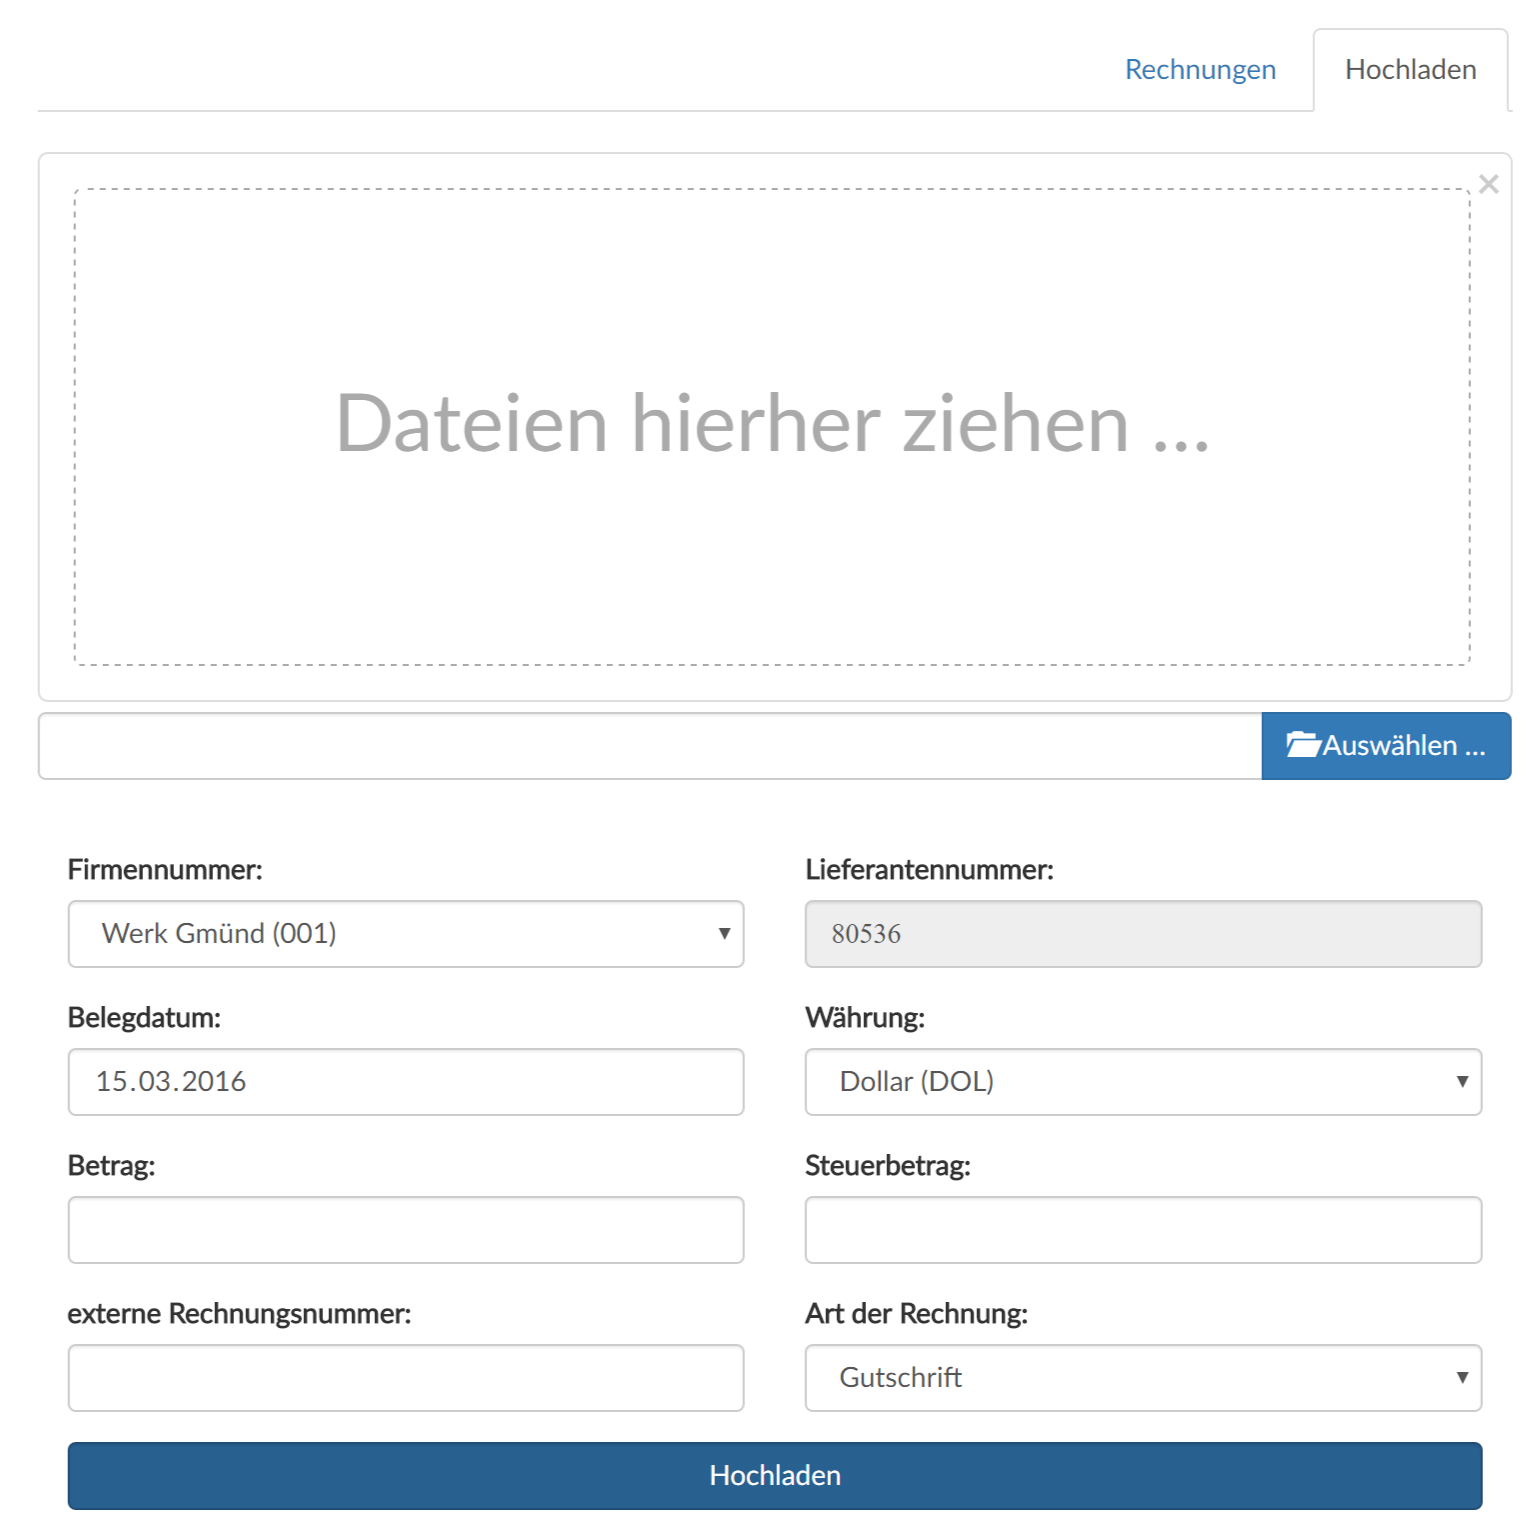
\includegraphics[width=310px, height=320px]{upload.png} & \\
\hline
\end{tabular}

\vspace{0.5cm}

\begin{tabular}{|p{53mm}|p{110mm}|@{}m{0cm}@{}}
\hline
Participation in \newline competitions \newline Awards & none & \\ 
\hline
\end{tabular}

\vspace{0.5cm}

\begin{tabular}{|p{53mm}|p{110mm}|@{}m{0cm}@{}}
\hline
Accessibility of \newline diploma thesis & HTL Krems Libary & \\
\hline
\end{tabular}

\vspace{0.5cm}

\begin{tabular}{|p{5.3cm}|p{5.28cm}|p{5.29cm}|@{}m{0cm}@{}}
\hline
\vspace{-0.6cm}Approval \newline (Date / Sign) & \vspace{-1.1cm} Examiner & \vspace{-1.1cm} Head of Department / \newline College & \\ [1.9cm]
\hline
\end{tabular}